\section{The ceiling on general-purpose code}
\label{sec:ceiling}

\textbf{Substrate and ground truth.} HumanEval+ and MBPP+ \citep{liu2023evalplus}: Python functions
with an executable hidden test suite. One frozen generator (\texttt{claude-haiku-4-5}) was shown each
specification and its visible tests and wrote one solution per problem, over two passes of 540
problems. A candidate that passes the visible suite and fails the hidden one is \emph{defective}; one
that passes both is \emph{correct}. Recall is measured on all 110 defective instances (56 problems)
and false positives on 150 correct ones drawn by seed. The auditor sees the specification, the
visible tests and the candidate, never the hidden suite. Because the defective stratum already
survived the visible tests, recall here is the fraction of that harder subset caught, not of all
defects a model writes (Appendix~\ref{sec:method}).

\textbf{Estimand and statistics.} Union recall at $K$: the fraction of defective instances blocked
(any finding graded BLOCKER) by at least one of $K$ independent readings, averaged exactly over all
size-$K$ subsets of the readings. The same union on correct instances is the false-positive rate,
always reported beside it (Table~\ref{tab:primary} collects the primary quantities). Intervals are 95\% problem-cluster percentile bootstraps; paired contrasts
carry exact McNemar and cluster sign-flip tests. The shipped cross-vendor route
(\texttt{gpt-5.6-terra}) sends no sampling parameter; same-vendor routes are sent temperature 0, a
difference that bounds every cross-family union contrast (Section~\ref{sec:auditor}).

\begin{figure*}[t]
\centering
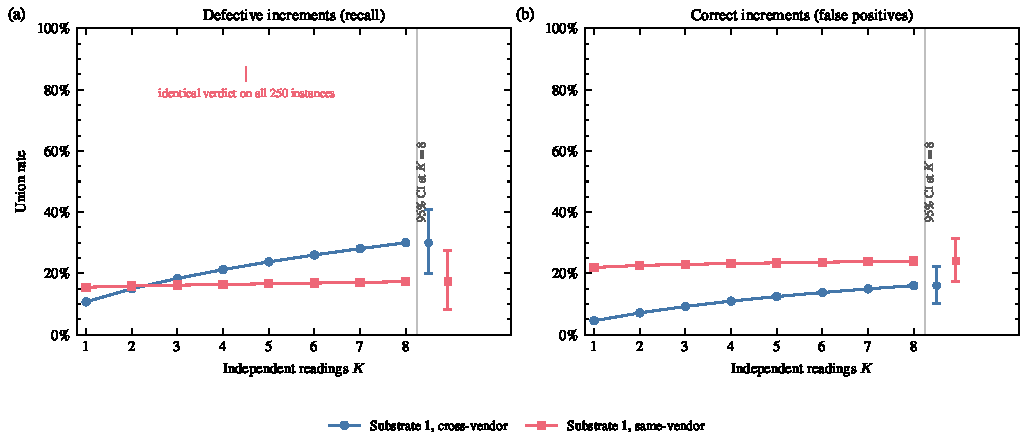
\includegraphics[width=\textwidth]{fig1_saturation.pdf}
\caption{\textbf{Returns to repeated reading diminish short of complete.} Union rate against the
number of independent readings $K$, for two auditor families. (a) Recall on defective instances;
(b) false positives on correct instances. Bars at the right of each panel give the 95\%
problem-cluster bootstrap interval of each series at $K=8$, dodged in $x$ so overlapping intervals
stay separable. The cross-vendor curve does not meet the preregistered flattening bar (its
last-step gain is 1.93 points [1.14, 2.78] against a bar of 1.0) and is not described as
saturating. The same-vendor curve meets it, at 0.23 points, but that route is sent temperature
$0$ and its verdict varies across readings on only 3 of 110 defective instances under this
configuration, so its flatness is not evidence of exhausted headroom; whether it reflects the
sampling or the model is not separated here (Section~\ref{sec:auditor}).}
\label{fig:saturation}
\end{figure*}

\begin{table*}[t]
\caption{Selected primary quantities of the general-code studies (Section~\ref{sec:ceiling} and Appendix~\ref{sec:results}), with the population it is measured on and the label its source report gives it. Values are percentages or percentage points. Intervals are 95\% problem-cluster percentile bootstraps unless the label names another method. The coverage simulation of \S\ref{sec:stats} measures single-rate intervals only; the contrasts and the category-conditioned shares have no measured coverage. The two third-rater rows rest on labels from a rater that agreed with itself on 7 of 11 repeated items (6 problems). The correct-code row counts disagreement on inputs extracted from the findings; of the 20 flagged instances, 9 agreed on every extracted input and 9 yielded no valid input, which can be neither confirmed nor refuted.  Every row is read from a committed record by \texttt{figures/make\_table1.py}.}
\label{tab:primary}
\centering
\footnotesize\setlength{\tabcolsep}{4pt}
\begin{tabular}{@{}llrll@{}}
\toprule
quantity & population & value & interval & label \\
\midrule
Union recall, shipped route, $K=8$ & 110 defect, 56 problems & 30.0\% & $[20.0, 40.7]$ & preregistered \\
Union false positives, shipped, $K=8$ & 150 correct, 143 problems & 16.0\% & $[10.1, 22.3]$ & preregistered \\
Pooled union, 3 routes & 110 defect & 48.2\% & $[36.7, 60.0]$ & preregistered \\
\quad its false positives & 150 correct & 36.0\% & $[28.2, 44.2]$ & derived (C1) \\
Gain from the eighth reading & 110 defect & $+1.93$ & $[1.14, 2.78]$ & bar 1.0, not met \\
Same-vendor stronger $-$ cross, recall & 110 defect & $-26.4$ & $[-37.3, -15.6]$ & preregistered \\
\quad its false-positive difference & 150 correct & $-12.7$ & $[-19.3, -6.1]$ & prereg.; 3.3\% v 16.0\% \\
Rulebook rule $-$ shipped, recall & 110 defect & $+30.9$ & $[+19.1, +43.1]$ & preregistered \\
\quad its false-positive cost & 150 correct & $+20.7$ & $[+12.8, +28.8]$ & preregistered \\
Rulebook rule, flags & 56 loop defect & $+26.8$ & $[+13.6, +40.4]$ & exploratory \\
\quad its cost on correct code & 56 loop correct & $+12.5$ & $[-3.6, +26.8]$ & unconditional, approx. \\
\quad isolating contrast, pass rate & 112 loop, 96 problems & $+5.4$ & $[-0.9, +12.1]$ & registered, failed \\
\texttt{astra} $-$ cross, common $K=4$ & 110 defect, 56 problems & $+11.5$ & $[+2.9, +21.3]$ & exploratory \\
\quad its false-positive difference & 150 correct & $-0.3$ & $[-3.8, +3.4]$ & exploratory \\
Undetermined, sheet groups & 121 entries, 110 instances & $+19.8$ & $[+1.2, +38.1]$ & registered method \\
\quad one definition of caught & 57 against 53 & $+23.3$ & $[+2.0, +43.6]$ & post hoc \\
Undetermined share, 3-family residual & 44 of 57 & 77.2\% & $[62.1, 91.1]$ & post hoc \\
\quad 6-family residual & 25 of 32 & 78.1\% & --- & post hoc (C14) \\
Correct-code flags, reference disagrees & 2 of 20 flagged & 10.0\% & $[0.0, 26.3]$ & preregistered (C16) \\
Clarified $-$ original, diagnosis & 32 selected, 19 problems & $+28.1$ & $[+7.7, +51.4]$ & one-signed; exact $p$ .0625 \\
\bottomrule
\end{tabular}
\end{table*}


\textbf{Repeated reading.} Union recall rises from 10.7\% at one reading to 30.0\% [20.0, 40.7] at
eight, at 16.0\% [10.1, 22.3] on correct code (Figure~\ref{fig:saturation}). The eighth reading still
adds 1.93 points [1.14, 2.78], above the 1.0-point flattening bar registered in advance, so we report
diminishing returns, not saturation. Twenty readings pooled across three families reach 48.2\%
[36.7, 60.0] at 36.0\% [28.2, 44.2] on correct code: pooling buys coverage at its own price.

\textbf{Which model reads.} Replacing the auditor with a stronger same-vendor model lowered union
recall at eight readings by 26.4 points [$-37.3$, $-15.6$] (exact McNemar $p = 4.2\times10^{-7}$;
cluster sign-flip $p = 2.0\times10^{-5}$), a preregistered primary. This is not a measure of auditing
ability. The stronger model also flags far less correct code, 3.3\% [0.7, 6.7] against 16.0\%, and
under an exploratory any-finding rule the sign reverses: 59.1\% [47.3, 70.6] recall at 34.0\%
[26.5, 41.7] on correct code, against 34.5\% [23.6, 45.5] at 19.3\% [12.8, 26.3]
(Figure~\ref{fig:sweep} in Appendix~\ref{sec:results}). At one reading, before the differently
sampled unions grow apart, the gap is only $-10.1$ points. A high-reasoning cross-vendor model reaches
32.7\% [20.7, 45.0] at 10.7\% [5.9, 16.1] with four readings, against the shipped route's 30.0\% at
16.0\% with eight, but no paired contrast establishes both advantages together.

\textbf{The rulebook.} We added one sentence to the auditor's rulebook: \emph{find what the visible
tests do not cover}. At one reading on 56 defective instances (41 problems), flags rose from 10 to
25, $+26.8$ points [13.6, 40.4] (exploratory; exact McNemar $p = 0.0003$, cluster sign-flip
$p = 0.0009$). On correct code they rose by 12.5 points, an interval [$-3.6$, $+26.8$] that includes
zero. An improvement in outcomes was not established: on the contrast that isolates the rule, the
hidden-suite pass rate after one revision moved $+5.4$ points [$-0.9$, $+12.1$]. The
sentence changes what the auditor writes; whether that makes code pass is not established.

\textbf{What is missed.} Fifty-seven of the 110 defective instances were flagged by no reading of
the first three families. Two model raters, one of them the agent that ran this programme, agree
post hoc that in 44 of them (77.2\% [62.1, 91.1]) the specification's prose does not settle the
value the hidden suite expects, as in the example that opens this paper. That reverses an earlier
classification of the same instances as unexercised edges. Being undetermined is not enough to be
missed: reading six families at forty readings shrinks the never-flagged set to 32 of 110, and 43
of the 68 instances both raters call undetermined are flagged by some reading. The undetermined
share of what remains is similar, 25 of 32 (78.1\%), but the 32 are a subset of the 57, so this is a
description, not a test of stability. Of twelve MBPP tasks an outside paper names as ambiguous,
incomplete or contradictory \citep{richter2026collapse}, 11 are in our defect population, and our
frozen labels call 9 of them undetermined (post hoc). An attempt to build a population whose
specifications determine the defect by construction did not deliver that property, so this
remains a post hoc description (Appendix~\ref{sec:inreview}).

\textbf{What follows.} A union recall figure is contingent on the false-positive rate it cost, the
model and sampling of the route, the rulebook, the decision rule, and what the benchmark's
specifications determine. Nine further studies, reported in Appendix~\ref{sec:inreview} with what
each licenses, include a specification-rewriting intervention that raised adjudicated diagnosis only
where the added rule did not wholly contradict the hidden suite, and a second substrate that closed without a
quotable number.
